\documentclass[12pt]{article}
\usepackage[utf8]{inputenc}
\usepackage{geometry}
\usepackage[T1]{fontenc}
\usepackage[spanish]{babel}
\usepackage{amsfonts}
\usepackage{afterpage}
\usepackage{graphicx}
\usepackage{float}
\usepackage{url}
\usepackage{hyperref}
\usepackage{enumerate}
\usepackage{bookmark}
\usepackage[sorting=none]{biblatex}
\usepackage{multirow}
\usepackage[table,xcdraw]{xcolor}
\usepackage{pgfgantt}
\usepackage{pgf}
\usepackage{xurl}
\usepackage{tabularray}
\usepackage{tabulary}
\usepackage{fancyhdr}
\usepackage[maxfloats=30,morefloats=12]{morefloats}
\usepackage{multicol}
\usepackage[dvipsnames]{xcolor}
\usepackage{awesomebox}
\usepackage{subcaption}
\usepackage{awesomebox}
\usepackage{pgfornament}
\usepackage[export]{adjustbox}
\usepackage{biblatex} %Imports biblatex package
\usepackage{tikzlings}
\usepackage{mathtools}
\DeclarePairedDelimiter\ket{\lvert}{\rangle}
\renewcommand{\labelenumi}{\textbf{\Roman{enumi})}} %Números romanos en mayúscula

\addbibresource{proyectotesis.bib} %Import the bibliography file
\fontfamily{put}\selectfont
\setlength{\columnsep}{40pt}
\setlength{\voffset}{0.5cm}
\setlength{\headsep}{40pt}
\setlength{\headheight}{34.06914pt} % Fix for fancyhdr error
\addtolength{\topmargin}{-22.06914pt} % Adjusted top margin as suggested by fancyhdr
\geometry{legalpaper, portrait, margin=2.3cm}

% Header and footer
\pagestyle{fancy}
\fancyhead[C]{
\includegraphics[width=0.05\textwidth]{images/escudo.png}}
\fancyhead[L]{\textbf{Proyecto de Tesis}\\ Universidad de Concepción}
\fancyhead[R]{\textbf{Florencia Fuentes}\\flofuentes2021@udec.cl}
\fancyfoot{}
% for adjust width environment
\usepackage[strict]{changepage}

% for formal definitions
\usepackage{framed}

\definecolor{morado1}{RGB}{106,27,154}
\definecolor{morado2}{RGB}{142,36,170}
\definecolor{rosa1}{RGB}{216,27,96}
\definecolor{rosa2}{RGB}{233,30,99}
\definecolor{lavanda}{RGB}{243,229,245}


% Definición de colores prolijos
\definecolor{violeto-claro}{RGB}{243, 229, 245} % Fondo de las barras
\definecolor{violeto-borde}{RGB}{149, 117, 205} % Bordes
\definecolor{violeto-oscuro}{RGB}{74, 20, 140}  % Texto y grupos
\definecolor{gris-linea}{RGB}{230, 230, 230}    % Cuadrícula suave


\definecolor{formalshade}{rgb}{.84, .69, .94}
%\definecolor{formalshade}{rgb}{.97, .88, .94}

\newenvironment{formal}{
  \def\FrameCommand{
    \hspace{1pt}
    {\color{White}\vrule width 2pt}
    {\color{Purple}\vrule width 4pt}
    \colorbox{formalshade!30!white}
  }
  \MakeFramed{\advance\hsize-\width\FrameRestore}%
  \noindent\hspace{-4.55pt}% disable indenting first paragraph
  \begin{adjustwidth}{}{7pt}%
  \vspace{2pt}\vspace{2pt}
}
{\vspace{2pt}\end{adjustwidth}\endMakeFramed}

\renewcommand{\headrulewidth}{0.1pt}

\usepackage{tikz}

\usepackage{tcolorbox}
\tcbuselibrary{minted}
\newtcblisting{mybox}{colback=white,minted language=latex,listing side text,righthand width=.5\textwidth}
\usetikzlibrary{ducks}
\usepackage{tikzducks}

%\definecolor{titlepagecolor}{cmyk}{0,.49,.15,.11}
\definecolor{titlepagecolor}{cmyk}{.11,.27,.0,.06}

\newcommand\titlepagedecoration{%
\begin{tikzpicture}[remember picture,overlay,shorten >= -10pt]

\coordinate (aux1) at ([yshift=-15pt]current page.north east);
\coordinate (aux2) at ([yshift=-410pt]current page.north east);
\coordinate (aux3) at ([xshift=-4.5cm]current page.north east);
\coordinate (aux4) at ([yshift=-150pt]current page.north east);

\begin{scope}[titlepagecolor!70,line width=12pt,rounded corners=12pt]
\draw
  (aux1) -- coordinate (a)
  ++(225:5) --
  ++(-45:5.1) coordinate (b);
\draw[shorten <= -10pt]
  (aux3) --
  (a) --
  (aux1);
\draw[opacity=0.6,titlepagecolor,shorten <= -10pt]
  (b) --
  ++(225:2.2) --
  ++(-45:2.2);
\end{scope}
\draw[titlepagecolor,line width=8pt,rounded corners=8pt,shorten <= -8pt]
  (aux4) --
  ++(225:0.8) --
  ++(-45:0.8);
\begin{scope}[titlepagecolor!70,line width=6pt,rounded corners=8pt]
\draw[shorten <= -10pt]
  (aux4) --
  ++(225:3) coordinate[pos=0.45] (c) --
  ++(-45:3.1);
\draw
  (aux4) --
  (c) --
  ++(135:2.5) --
  ++(45:2.5) --
  ++(-45:2.5) coordinate[pos=0.3] (d);   
\draw 
  (d) -- +(45:1);
\end{scope}
\end{tikzpicture}%
}

\DeclareFixedFont{\titlefont}{T1}{ppl}{b}{it}{0.5in}

\let\hrefWithoutArrow\href

\renewcommand{\href}[2]{\hrefWithoutArrow{#1}{\ifthenelse{\equal{#2}{}}{ }{#2 }\raisebox{.15ex}{\footnotesize \faExternalLink*}}}

%todo
\def\DefaultHeightofCheckBox{0.6\baselineskip}
\def\DefaultWidthofCheckBox{0.6\baselineskip}

\newcounter{checkcount}
\newcommand{\chk}{
    \stepcounter{checkcount} 
    \CheckBox[name=\thecheckcount, 
            bordercolor= Purple,backgroundcolor= Lavender!40!White]{} \hspace{1pt}}

\newenvironment{todolist}{
    \begin{list}{\chk}
            {\setlength{\parsep}{0pt plus2pt minus1pt} 
            \setlength{\labelsep}{1pt} }
            }
    {\end{list}}


\begin{document}
% ==============================================================================
% Title
% ==============================================================================


% environment derived from framed.sty: see left bar environment definition
\pagecolor{Fuchsia!30!White}\afterpage{\nopagecolor}
%\maketitle

\begin{titlepage}
    \centering

    
\includegraphics[width=0.2\textwidth,left]{images/escudo.png}

    \vspace*{5cm}

    {\Huge\bfseries Optimización de Tapered Amplifiers \par}

    \vspace{0.2cm}

    {\raggedleft\Large\itshape Proyecto de Tesis \qquad  \par}

    \vfill


    {\Large \bfseries Florencia Fuentes Jara \par} 

    
    \vspace{0.1cm}

    \mbox{\hrefWithoutArrow{mailto:flofuentes2021@udec.cl}{\color{VioletRed}{\footnotesize\faEnvelope[regular]}\hspace*{0.13cm}flofuentes2021@udec.cl}}%

    \vspace{0.5cm}
    {\large Profesor Guía: Pablo Solano Palma \par}

    \vspace{1cm}

    {\large
    Universidad de Concepción\\
    Faculty of Physical and Mathematical Sciences\\
    Department of Physics
    \par}

    \titlepagedecoration
\end{titlepage}

\thispagestyle{fancy}
\newpage
% Table of Contents
\tableofcontents
\thispagestyle{fancy}

\clearpage

% Begin page numbers
\fancyfoot[C]{\thepage}
\pagenumbering{arabic}

% ===============================
% SUMMARY SECTION
% ===============================
\section{Resumen}
%\addcontentsline{toc}{section}{Resumen}
Este proyecto de tesis se centra en el desarrollo, caracterización y optimización de un sistema láser de alta potencia basado en la configuración Master Oscillator Power Amplifier(MOPA). El sistema consiste en la integración de un láser de diodo de cavidad externa (ECDL) como oscilador maestro y un amplificador cónico (Tapered Amplifier) como etapa de potencia. El objetivo principal es obtener una fuente de luz que mantenga la estabilidad espectral y el estrecho ancho de línea del ECDL con una elevada potencia de salida dada por el TA, características fundamentales para el desarrollo de experimentos de física atómica y óptica cuántica, como el enfriamiento y atrapamiento de átomos. 

A través de un abordaje experimental, se caracterizarán los parámetros de salida ($P_{out}$) en función de la corriente, temperatura y potencia de entrada, además de realizar un análisis de la calidad del haz mediante la medición del parámetro $M^2$ y espectroscopía heterodina. Los resultados esperados permitirán establecer un protocolo de optimización que garantice la estabilidad del sistema y la ausencia de saltos de modo en regímenes de alta potencia.
% ===============================
% INTRODUCTION SECTION
% ===============================
\section{Introduction}

Los amplificadores ópticos son dispositivos fundamentales en el área de fótonica ya que reciben una señal de luz de entrada y generan una señal de salida con mayor potencia óptica. La mayoría de los amplificadores ópticos son amplificadores láser donde la amplificación se basa en la emisión estimulada, proceso que ocurre en un medio de ganancia que debe ser bombeado por una fuente externa, ya sea ópticamente o electrónicamente.
\\ \newline
Los sistemas láser de amplificador cónico (tapered amplifier, TA) son esenciales en muchos experimentos de física atómica moderna y óptica cuántica, así como en aplicaciones de comunicación que requieren alta potencia\cite{articlechi}. Estos sistemas permiten la amplificación de láseres de diodo de cavidad externa (ECDL) para producir grandes potencias ópticas manteniendo estrecha la anchura de línea del láser semilla.
\\ \newline
Mientras que los ECDL son comúnmente utilizados debido a su bajo costo, efectividad y precisión, estos láseres son solo capaces de producir potencias de salida menores a 100 mW \cite{Wang}. Por esta razón, un amplificador que produzca grandes ganancias ópticas preservando el estrecho ancho de línea del ECDL es esencial para enfriar átomos en experimentos de física atómica. El amplificador cónico (TA) es un dispositivo común utilizado para este efecto.

%Motivación: Diodos baja Potencia de salida para AMO necesitamos una potencia de salida mayor. -> solución :TA

% ===============================
% THEORY SECTION
% ===============================

\section{Estado del arte y Marco Teórico}
La finalidad del proyecto de tesis es desarrollar y optimizar un sistema láser de amplificador cónico (TA) acoplado a un láser de diodo de cavidad externa (ECDL) para aplicaciones en física atómica, mejorando la calidad espectral, la potencia de salida y la sintonización sin saltos de modo. Este marco teórico establece las bases de dichos componentes y los parámetros de caracterización fundamentales.

\subsection{¿Qué es un Tampered Amplifier?}
Los amplificadores cónicos (TA) son amplificadores ópticos con una sección cónica, donde el área transversal del haz amplificado aumenta gradualmente. Nos centramos en dispositivos semiconductores cónicos, disponibles como chips semiconductores simples o como módulos amplificadores que contienen dichos chips. Pueden producir potencias de salida de varios Watts manteniendo una alta calidad del haz \cite{Paschotta_2019_tapered_amplifiers}.

\begin{formal}
\textbf{Amplificadores Ópticos:} Dispositivo que recibe una señal de luz entrante y produce una señal de salida con más potencia óptica. La amplificación tiene lugar en un "gain medium" que debe ser bombardeado por una fuente externa (óptica o electrónica).
\end{formal}

\subsection*{Chip TA}
El chip TA está compuesto por una sección de guía con un índice (L1) que es corta y recta, la cual se encuentra acoplada a una sección cónica más larga que tiene una guía de ganancia (L2). La luz se introduce por una estrecha apertura (W1) de la sección que tiene una guía de índice. La Figura \ref{fig:TAchip} ilustra que la salida amplificada se emite a través de la abertura mucho más amplia (W2) de la sección cónica con guía de ganancia.

\begin{figure}[H]
  \centering
  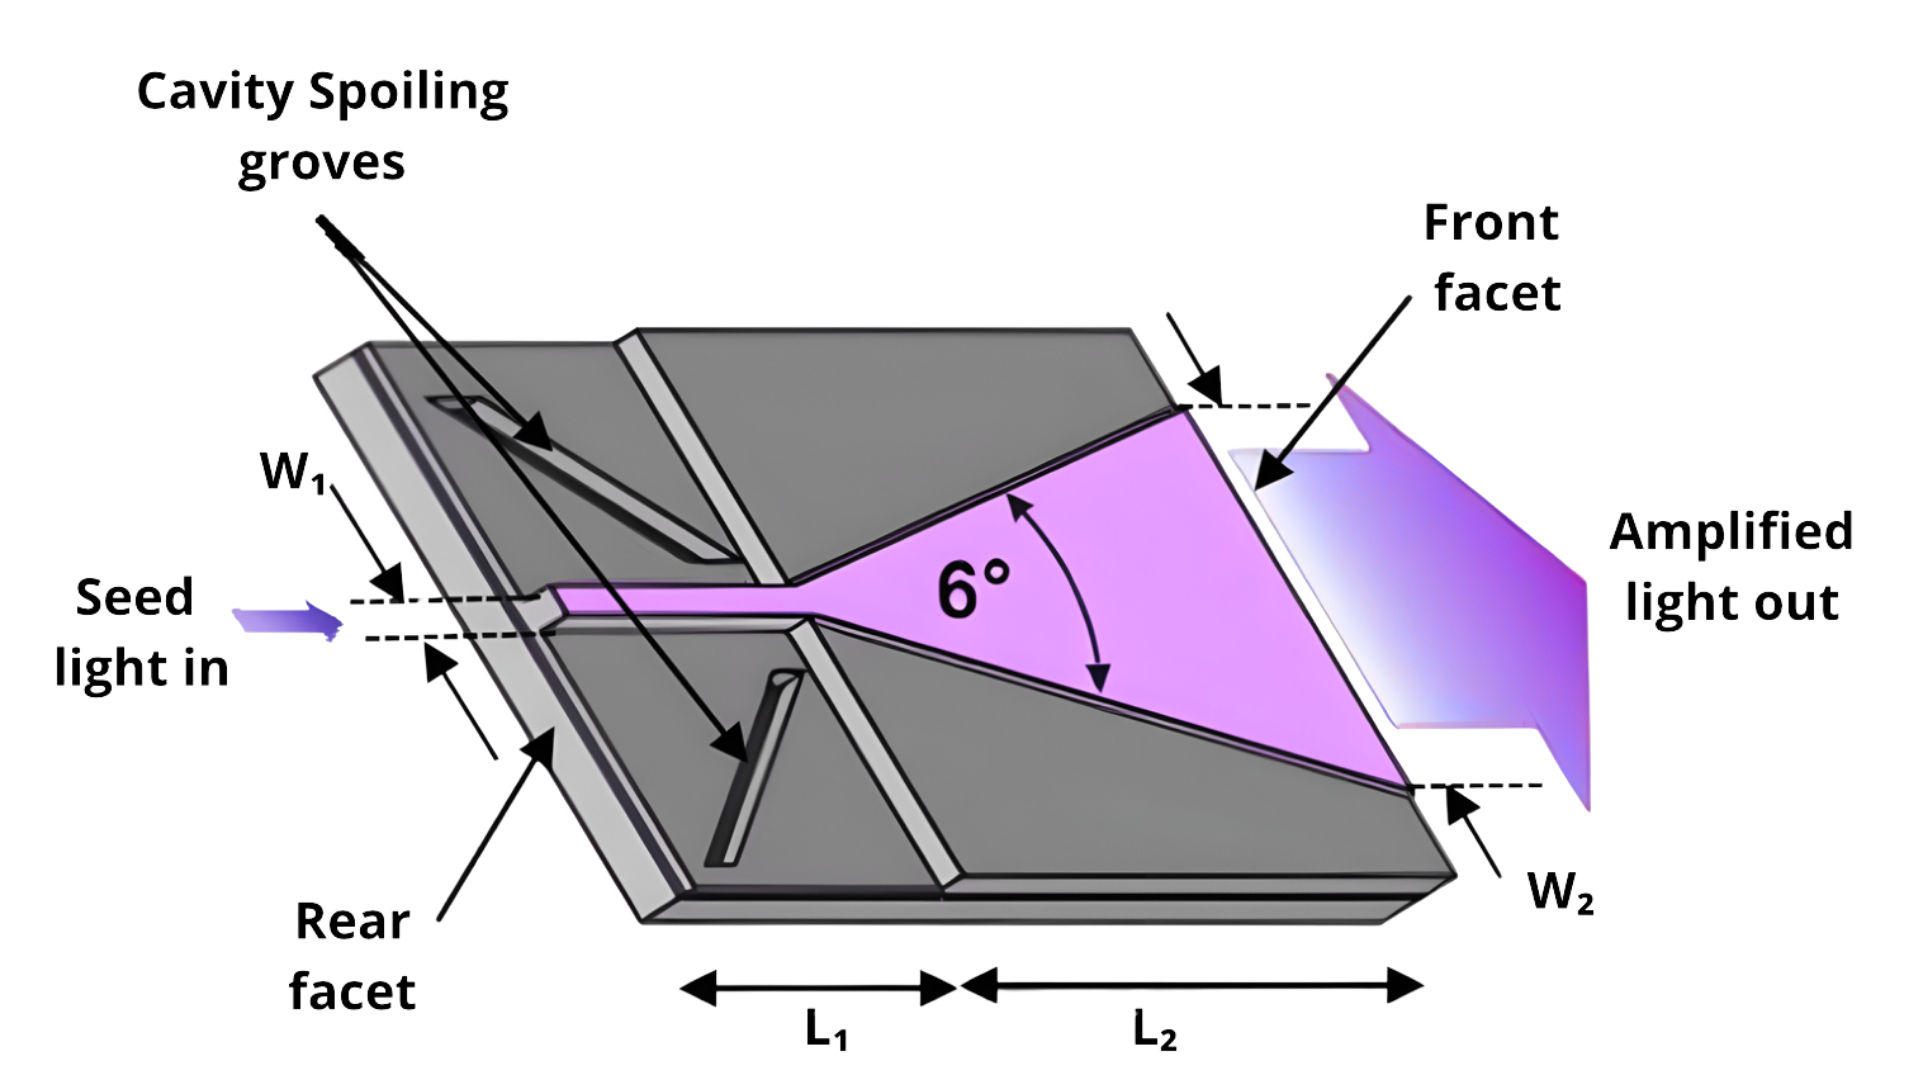
\includegraphics[width=0.7\linewidth]{Images/TAchip.png}
  \caption{Esquema de un chip TA}
  \label{fig:TAchip}
\end{figure}

El diseño del chip del amplificador cónico puede considerarse como consistente de dos componentes principales: una guía de onda y una región de ganancia cónica. La luz del ECDL  entra al amplificador a través de una faceta recubierta con un revestimiento anti-reflectante y llena la guía de onda. La faceta de entrada de la guía de onda es de solo de $\mu m$ de ancho, lo que permite que pequeñas cantidades de potencia de entrada creen grandes densidades de energía dentro de la guía de onda \cite{10.1117/12.697935}.
\\  \newline
Después de propagarse por la guía de onda, la luz  alcanza la región cónica y se difracta para llenar completamente la región de ganancia. Esta región es bombeada uniformemente por una corriente externa, que proporciona la energía para facilitar la amplificación. El resultado es un amplificador de paso único de alta potencia donde un oscilador maestro de modo único (MO) se inyecta en una región de ganancia que se expande lateralmente, de modo que la potencia óptica se amplifica mientras el modo lateral se expande hacia una salida cónica de gran área, permitiendo alta potencia de salida con propiedades espectrales preservadas del MO \cite{10.1117/12.2288337}.

\subsection{¿Comó funciona?: Principio físico del TA}

Para analizar el proceso de amplificación de un fotón semilla, el medio de ganancia puede considerarse un sistema de dos estados, con un estado basal $\ket{A}$ y un estado exicitado $\ket{B}$ . Cuando el medio es bombeado por una corriente de excitación, los electrones en el estado $\ket{A}$ se excitan al estado superior $\ket{B}$. Mediante este proceso, se crea una inversión de población, en la que se encuentran más electrones en el estado superior que en el inferior. Una vez en el estado superior, los electrones pueden decaer de nuevo al estado $\ket{A}$ mediante procesos espontáneos o estimulados. Cuando un electrón está en el estado $\ket{B}$, puede decaer estocásticamente al estado $\ket{A}$ y emitir un fotón. Dado que el fotón emitido no está causalmente vinculado a los fotones semilla, el modo de los dos fotones no coincide necesariamente . Por el contrario, cuando el sistema se encuentra en el estado $\ket{B}$, un fotón del láser semilla puede estimular una desintegración al estado $\ket{A}$, emitiendo de nuevo un fotón. Dado que el fotón semilla estimula la creación del segundo fotón, ambos fotones deben tener modos idénticos. Esto garantiza que la frecuencia, la dirección de propagación y la polarización de ambos fotones sean idénticas. El resultado neto de este proceso es la creación de dos fotones a partir de un único fotón semilla. En la Figura \ref{fig:TAteory} se muestra un esquema de estos procesos.
\\  \newline
Luego los fotones involucrados en los procesos estimulados o estocásticos continúan propagándose a través del medio de ganancia y son libres de estimular nuevas transiciones y emisiones.Sin embargo, dado que los fotones producidos en la emisión estimulada coinciden con el modo del láser de semilla, pueden considerarse el único producto útil del proceso de amplificación. A medida que estos fotones se propagan a través del medio de ganancia, crean una avalancha  de fotones idénticos, todos creados a partir de una única partícula incidente. Este efecto de avalancha es el mecanismo por el cual el amplificador cónico amplifica la luz incidente. \cite{DigitalCommonsColby}

\begin{figure}[H]
  \centering
  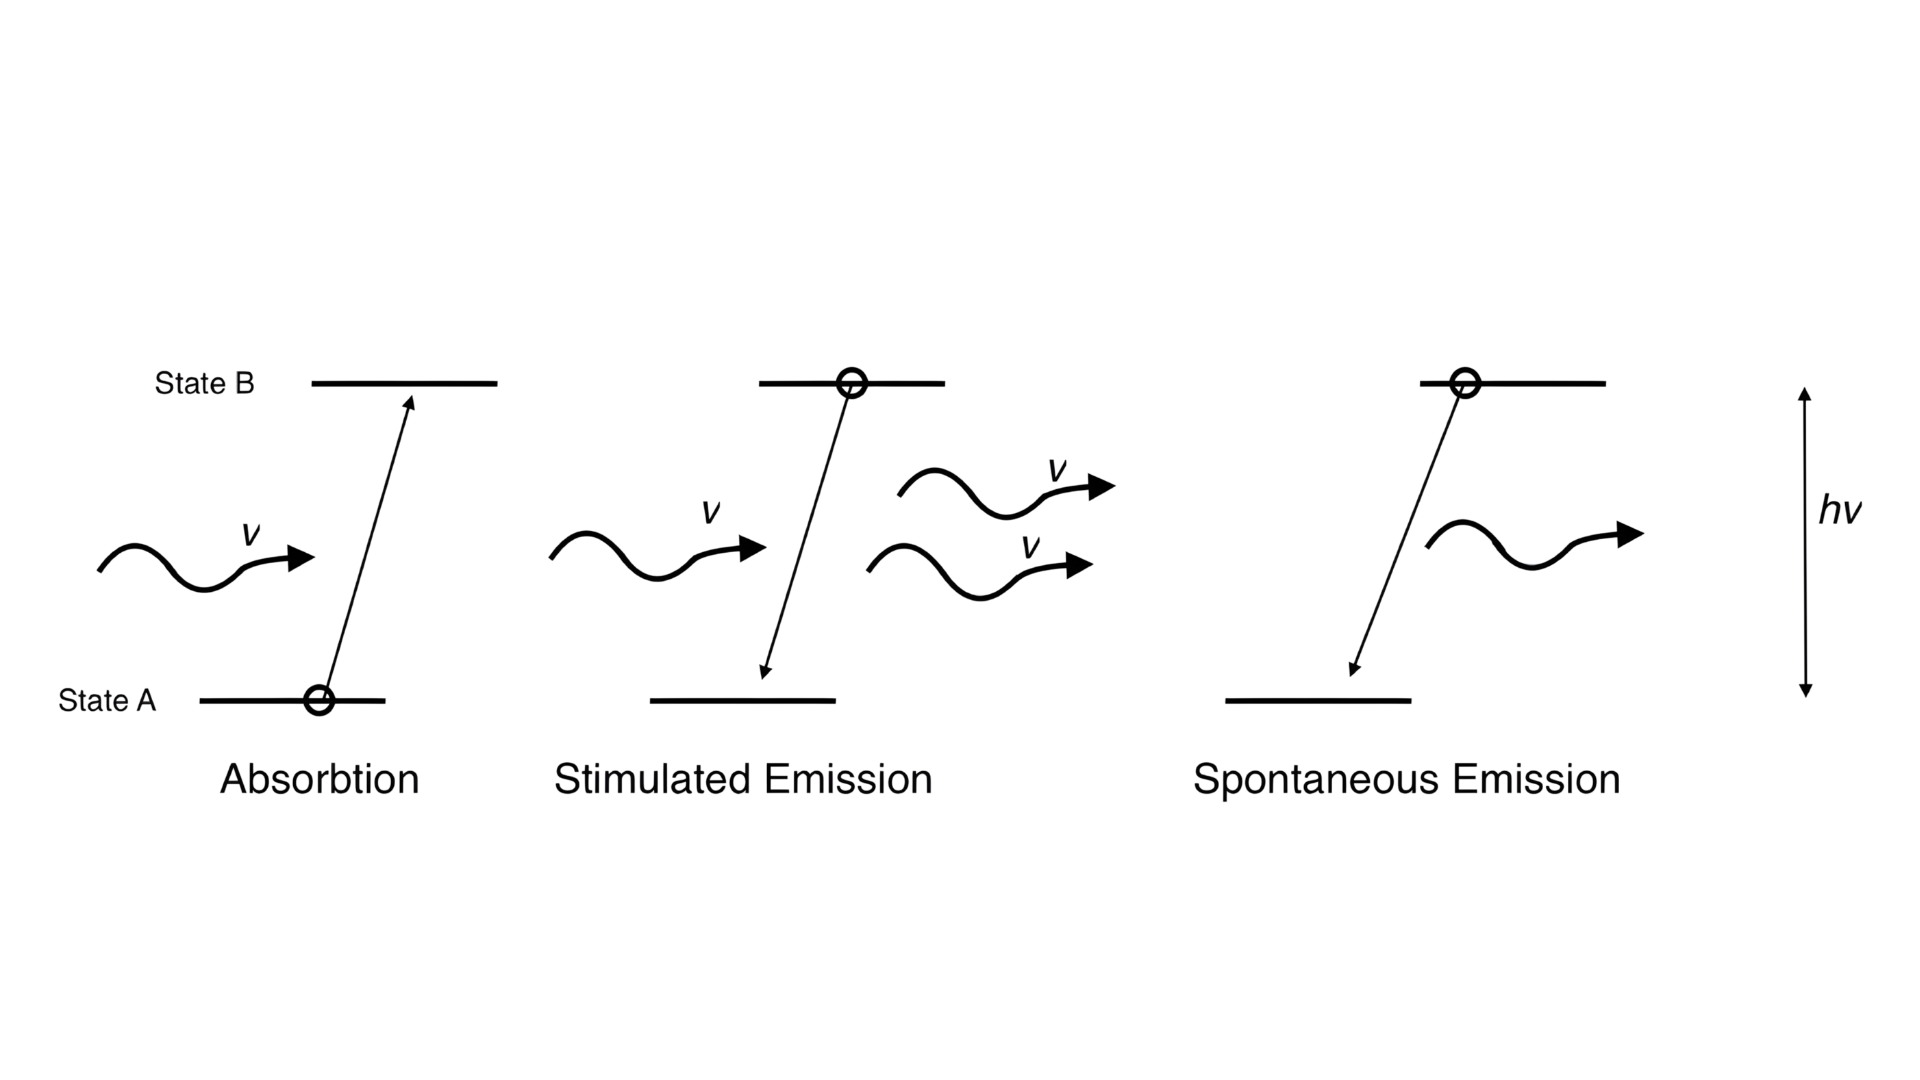
\includegraphics[width=0.9\linewidth]{Images/TAteory.png}
  \caption{Diagrama de niveles de energía que muestra los procesos involucrados en el modelo de dos niveles del amplificador cónico.}
  \label{fig:TAteory}
\end{figure}


\subsection{¿Qué es un Master Oscillator Power Amplifier (MOPA)?}
El término amplificador de potencia del oscilador maestro (MOPA) se refiere a una configuración que consta de un láser maestro o láser de semilla y un amplificador óptico para aumentar la potencia de salida. En este caso, un MOPA consta de un láser de diodo de cavidad externa sintonizable y un amplificador óptico semiconductor \cite{Paschotta_2005_master_oscillator_power_amplifier}.

\section{Objetivos}
El proyecto tiene como objetivo general optimizar el funcionamiento de los TA’s disponibles en el laboratorio, aumentando la potencia de los láseres mientras se mantiene la calidad del haz y la estabilidad espectral. Los objetivos específicos incluyen:

\subsection*{Montaje del Sistema Experimental}

\begin{todolist}
  \item Montar el setup experimental completo para la caracterización de TA.
  \item Alinear los componentes ópticos.
  \item Acoplar el sistema como si fuera una fibra.
\end{todolist}

\subsection*{Caracterización de Parámetros de Salida}
\begin{todolist}
\item Caracterizar la potencia de salida ($P_{out}$) en función de:

\begin{todolist}
  \item Potencia de entrada ($P_{in}$):
  \begin{itemize}
    \item[]  Realizar barridos de potencia de entrada para medir el comportamiento de ganancia del amplificador y saturación
  \end{itemize}
  \item Corriente ($I$): 
  \begin{itemize}
    \item[] Registrar curvas de potencia de salida versus la corriente del amplificador a condiciones  fijas para determinar la eficiencia de pendiente, comportamiento tipo umbral de las facetas, y el inicio de inestabilidades espaciales.
  \end{itemize}
  \item Temperatura de operación ($T$):
  \begin{itemize}
    \item [] Medir potencia de salida, espectro y perfil del haz a través del rango de temperatura operacional para evaluar el desplazamiento de longitud de onda, movimiento del peak de ganancia, y rollover térmico.
  \end{itemize}
\end{todolist}
\end{todolist}
%porque optimizar
\section{Metodología}
La finalidad de este proyecto de tesis es desarrollar y optimizar un sistema láser de amplificador cónico (TA) acoplado a un sistema láser de diodo de cavidad externa (ECDL), centrándose en mejorar la calidad espectral, la potencia de salida y la capacidad de sintonización sin saltos de modo para aplicaciones en experimentos de física atómica.
\\ \newline
La investigación se fundamentará en un diseño experimental de mediciones repetidas, donde la corriente $(I)$, temperatura de operación $(T)$, y potencia de entrada$(P_{in})$ serán manipuladas de manera sistemática para evaluar su efecto sobre la potencia de salida $(P_{out})$. La metodología a utilizar seran descritas por las siguientes fases:
\begin{enumerate}
  \item \textbf{Configuración y Caracterización del Sistema:}
  \begin{enumerate}[$\bullet$] 
    \item Montaje del arreglo experimental en configuración MOPA (Master Oscillator Power Amplifier), empleando un láser de diodo de cavidad externa (ECDL) como oscilador maestro y el amplificador cónico como elemento de potencia.
    \item Alineación óptica mediante visualización del haz con tarjeta de visualización, seguido del acoplamiento del haz semilla a la entrada del amplificador utilizando lentes asféricas y monturas de ajuste.
  \end{enumerate}
  \item \textbf{Caracterización Paramétrica:}
  Realización de tres series de mediciones fundamentales:
  \begin{enumerate}[a)]
    \item \textbf{Curvas de luz-corriente (L-I):} Se registrará la potencia óptica de salida en función de la corriente aplicada al amplificador con el objetivo de determinar la eficiencia de pendiente, identificar regiones de operación lineal, y detectar posibles inestabilidades.
    \item  \textbf{Curvas de ganancia y saturación ($P_{out}$ vs $P_{in}$):} Variación de la potencia del láser semilla desde valores de $\mu W$ hasta el régimen de saturación del amplificador, lo que permitirá cuantificar la ganancia de pequeña señal (small-signal gain), la potencia de saturación de salida, y el régimen dinámico del amplificador.
    \item \textbf{Caracterización térmica ($P_{out}$ vs $T$)}:Mediciones de potencia de salida, espectro óptico y perfil espacial del haz mientras se varía la temperatura del montaje del chip amplificador en un rango típico de 15°C a 35°C.
  \end{enumerate}
  \item \textbf{Caracterización Avanzada de Calidad del Haz:}Se implementarán técnicas para evaluar la propagación de la luz amplificada.
  \begin{enumerate}[$\bullet$]
    \item Se usará el método de variación del radio del haz (beam waist scanning) para determinar el parámetro $M^2$ según la norma ISO 11146, midiendo el diámetro del haz con un perfilador de haz CCD. 
    \item Se realizarán mediciones de distribución de intensidad en campo lejano proyectando el haz en una pantalla difusora o usando una lente de Fourier, calculando la fracción de energía en el lóbulo central y evaluando distorsiones modales. Se compararán los perfiles modales de entrada y salida mediante análisis de frente de onda y propagación numérica, evaluando la fidelidad de amplificación modal. 
    \item Se llevará a cabo una caracterización espectral de alta resolución mediante espectroscopía heterodina para verificar la preservación del ancho de línea del ECDL tras la amplificación y detectar posibles contribuciones de emisión espontánea amplificada.
  \end{enumerate}
  \item \textbf{Análisis de Datos:} Los datos experimentales se procesarán y analizarán con software especializado para realizar ajustes de curvas, análisis estadístico y visualización gráfica, utilizando Python o MATLAB, lo que facilitará la extracción de parámetros físicos y la creación de representaciones visuales de los resultados.
\end{enumerate}

Finalmente, los hallazgos experimentales serán interpretados en el contexto del marco teórico establecido y se formularán recomendaciones específicas para aplicaciones futuras del sistema optimizado en experimentos de enfriamiento y atrapamiento atómico. Esta metodología garantiza un abordaje sistemático, reproducible y científicamente riguroso del problema de investigación, permitiendo no solo la optimización práctica del sistema experimental disponible en el laboratorio, sino también la generación de conocimiento fundamental sobre los mecanismos físicos que gobiernan el desempeño de amplificadores cónicos en régimen de alta potencia.Los plazos y la secuencia de estas fases se detallan en la Figura \ref{fig:gantt2026}


%montar setup 
%caracterizar Pout en funcion de Pin, I y T
\section{Carta Gantt}

\begin{figure}[H]
\centering
\begin{ganttchart}[
    % --- Dimensiones ---
    expand chart=\textwidth, % Ajusta al ancho de página
    y unit title=0.6cm,
    y unit chart=0.6cm,
    % --- Estilo de Cuadrícula (más sutil) ---
    vgrid={*1{gris-linea, thin}},
    hgrid={*1{gris-linea, thin}},
    % --- Títulos ---
    title height=1,
    title label font=\small\bfseries\color{white},
    title/.style={fill=violeto-oscuro!80!white, draw=gris-linea},
    % --- Estilo de Barras (Violeta Claro solicitado) ---
    bar/.append style={fill=violeto-claro, draw=violeto-borde, rounded corners=2pt},
    bar height=0.5,
    bar left shift=0.1,
    bar right shift=-0.1,
    bar label font=\footnotesize\color{black!80},
    % --- Estilo de Grupos ---
    group/.append style={fill=violeto-oscuro!40!white, draw=violeto-oscuro},
    group left shift=0.1,
    group right shift=-0.1,
    group top shift=0.25,
    %group right peak width =0.4,
    %group right peak height = 0.1,
    group peaks tip position=0.5,
    group peaks height=0,
    group height=0.3,
    group label font=\small\bfseries\color{violeto-oscuro},
    % --- Otros ---
    milestone/.append style={fill=violeto-oscuro, draw=violeto-oscuro},
    milestone label font=\color{violet},
    %progress label text={} % Quita porcentajes si no se usan
]{1}{12}

% Encabezado de Meses
\gantttitle{Plan de Trabajo 2026}{12} \\
\gantttitlelist{1,...,12}{1} \\

% --- Bloque 1 ---
\ganttgroup{Revisión Bibliográfica}{1}{2} \\
\ganttbar{Análisis de literatura}{1}{2} \\


% --- Bloque 2 ---
\ganttgroup{Fase I: Configuración y Caracterización del Sistema}{3}{3} \\
\ganttbar{Montaje ECDL + TA}{3}{3} \\
\ganttbar{Alineación y acoplamiento}{3}{3} \\

% --- Bloque 3 ---
\ganttgroup{Fase II: Caracterización Paramétrica}{4}{6} \\
\ganttbar{Curvas L-I }{4}{4} \\
\ganttbar{Curvas de ganancia y saturación}{5}{5} \\
\ganttbar{Caracterización térmica}{6}{6} \\

% --- Bloque 4 ---
\ganttgroup{Fase III: Caracterización Avanzada de calidad de Haz}{7}{9} \\
\ganttbar{Medición M$^2$ }{7}{7} \\
\ganttbar{Análisis modal}{8}{8} \\
\ganttbar{Espectroscopía}{9}{9} \\

% --- Bloque 5 ---
\ganttgroup{Fase IV: Escritura}{10}{11} \\
\ganttbar{Análisis de Datos}{10}{10} \\
\ganttbar{Redacción de informe}{7}{11} \\
\ganttmilestone{Entrega Borrador}{11}

\end{ganttchart}
\caption{Carta Gantt 2026}
\label{fig:gantt2026}
\end{figure}

\section{Antecedentes}
La ejecución exitosa de este proyecto se sustenta en una sólida base de experiencias previas en el laboratorio. En particular el  desarrollo de sistemas de reducción de ancho de línea para diodos láser fabricados en casa. Esta experiencia previa permitió adquirir destrezas en el manejo de cavidades externas, control de retroalimentación óptica y estabilización de frecuencia, competencias que son directamente transferibles al montaje y optimización del setup MOPA propuestó en este plan.

Además el proyecto cuenta con el apoyo integral del equipo en el \textbf{Laboratorio de física átomica y molecular (LAMP)}. Donde la colaboración directa con investigadores experimentados en el área, garantiza la disponibilidad de recursos ópticos de alta calidad y el soporte teórico experimental necesario para solucionar eventuales problematicas durante las fases de montaje y caracterización avanzada. 
%  Novedad científica

% ===============================
% RESULTS SECTION
% ===============================
\section{Conclusiones}
 
Esta tesis busca aportar al saber práctico y teórico sobre la optimización de amplificadores cónicos para su uso en experimentos de física atómica y óptica cuántica. Se espera que la implementación de métodos de optimización fundamentados en la literatura actual y una caracterización sistemática logren aumentar significativamente el desempeño de los amplificadores cónicos que están disponibles en el laboratorio. Se espera que los resultados incluyan una caracterización integral de los parámetros de rendimiento, cuantificación del haz de calidad.
Contribuyendo al progreso de fuentes láser que sean de mayor calidad y potencia para la realización de experimentos atómicos en el laboratorio.


\vfill
\begin{flushright}
    \begin{tikzpicture}
        \duck[body=violet!40!white, unicorn=magenta!60!violet, longhair=magenta!60!violet, signpost=\parbox{2cm}{\tiny\color{black}\centering Bye! }, signcolour=brown!70!gray, signback=white!80!purple, shift={(2.5,0)}]      
\end{tikzpicture}
\end{flushright}

\newpage
% ===============================
% REFERENCES SECTION
% ===============================
\section*{Referencias}
\addcontentsline{toc}{section}{Referencias}
% Add your bibliography entries here
%\nocite{*}
\printbibliography[heading=none]
% ===============================
\vfill
\begin{center}
    \begin{tikzpicture}
        \bee[cocktail,think={\small\color{black}\centering Thanks!}, bubblecolour=gray!30!white
]      
   \end{tikzpicture}
\end{center}


\end{document}
